
% File acl2020.tex
%
%% Based on the style files for ACL 2020, which were
%% Based on the style files for ACL 2018, NAACL 2018/19, which were
%% Based on the style files for ACL-2015, with some improvements
%%  taken from the NAACL-2016 style
%% Based on the style files for ACL-2014, which were, in turn,
%% based on ACL-2013, ACL-2012, ACL-2011, ACL-2010, ACL-IJCNLP-2009,
%% EACL-2009, IJCNLP-2008...
%% Based on the style files for EACL 2006 by 
%%e.agirre@ehu.es or Sergi.Balari@uab.es
%% and that of ACL 08 by Joakim Nivre and Noah Smith

\documentclass[11pt,a4paper]{article}
\usepackage[hyperref]{acl2020}
\usepackage{times}
\usepackage{graphicx}
\usepackage{latexsym}
\usepackage{float}
\usepackage{placeins}
\usepackage{booktabs}
\renewcommand{\UrlFont}{\ttfamily\small}

% This is not strictly necessary, and may be commented out,
% but it will improve the layout of the manuscript,
% and will typically save some space.
\usepackage{microtype}

\aclfinalcopy % Uncomment this line for the final submission
%\def\aclpaperid{***} %  Enter the acl Paper ID here

%\setlength\titlebox{5cm}
% You can expand the titlebox if you need extra space
% to show all the authors. Please do not make the titlebox
% smaller than 5cm (the original size); we will check this
% in the camera-ready version and ask you to change it back.

\newcommand\BibTeX{B\textsc{ib}\TeX}

%%%%%%%%%%%%%%%%%%%%%%%%%%%%%%%%%%%%%%%%%%%%%%%%%%%%

\title{Hw1: Presidential Speech Classification with Word Embeddings}

\author{Sam Showalter \\
  University of California, Irvine \ (showalte) \\  
  Kaggle: Sam Showalter \\
\texttt{showalte@uci.edu}} 

\date{}

%%%%%%%%%%%%%%%%%%%%%%%%%%%%%%%%%%%%%%%%%%%%%%%%%%%%

\begin{document}
\maketitle
\begin{abstract}
  Text classification in model-restrictive settings is heavily reliant on predictive features to ensure adequate performance. In turn, this analysis explores several methods of text tokenization, feature engineering, and dimensionality reduction. Starting with simple dataset exploration, our experiments extend to attempts at encoding semantic meaning into the naive bag-of-words representations with Truncated Singular Value Decomposition and Word2Vec embeddings.
  Moreover, this experimentation was also applied to the model itself. Since the input features from the speeches are high-dimensional, different regularization methods were applied to improve learning and generalization. After each ablation, performance on a held-out validation set improved, and the best configuration from the experiment was passed to the next and built upon progressively. 
  In addition, we further improved our classification performance by pretraining an embedding model on unlabeled data with Word2Vec, correlating words based on their meaning. Though alone these word embeddings did not exceed the supervised performance, when integrated the original set of supervised features performance improved slightly. However, the embeddings did exhibit a few failure modes where context hurt; these issues were be tracked back to the structure of the unlabeled data.  
\end{abstract}


%%%%%%%%%%%%%%%%%%%%%%%%%%%%%%%%%%%%%%%%%%%%%%%%%%%%
% Introduction
%%%%%%%%%%%%%%%%%%%%%%%%%%%%%%%%%%%%%%%%%%%%%%%%%%%%
\section{Introduction}

Text classification can be accomplished with a variety of implementations. Among the simplest and most popular is the bag-of-words framework \cite{zhang2010understanding}. In this setting, a vocabulary is formed by tokenizing the input text and then creating a unique index for every distinct token. Then, one-hot vectors of each token are generated and a document's feature vector is represented as the sum or the logical-OR of its token vectors.

In general, feature vectors for NLP tend to be high-dimensional. To combat this curse of dimensionality in modeling, the vocabulary can be shrunk by several methods, including removing non-alphanumeric characters, expanding contractions, lemmatization, and removing stopwords. Even with these reductions, the resulting feature vectors tend to remain quite large. Further explicit reductions can come from recognizing that tokens that occur extremely rarely likely carry little predictive value. However, There is no guarantee this is true.

In subsequent sections, we outline our approach to feature engineering, supervised learning, and incorporating unlabeled data. Our main experimental contributions can be defined as follows:
\begin{enumerate}
  \vspace{-2mm}
  \item We extensively explore feature engineering pipelines, including tokenization creation and resolution methods.
  \vspace{-2mm}
    \item We explore dimensionality reduction techniques with and without the use of unlabeled data with Truncated SVD and Word2Vec.
  \vspace{-2mm}
      \item We regularize our model, Logistic Regression, in several different ways and apply different gradient based solvers to the optimization.
  \vspace{-2mm}
\end{enumerate}




%%%%%%%%%%%%%%%%%%%%%%%%%%%%%%%%%%%%%%%%%%%%%%%%%%%%
% Supervised Learning Grid Search
%%%%%%%%%%%%%%%%%%%%%%%%%%%%%%%%%%%%%%%%%%%%%%%%%%%%
\section{Supervised Learning}%
\label{sec:supervised_learning}

In this section, we discuss methods of improving classification performance without making use of unlabeled data. The following sections are separated by feature- and model-based exploration.


%%%%%%%%%%%%%%%%%%%%%%%%%%%%%%%%%%%%%%%%%%%%%%%%%%%%
% Feature Engineering
%%%%%%%%%%%%%%%%%%%%%%%%%%%%%%%%%%%%%%%%%%%%%%%%%%%
\subsection{Feature Engineering}%
\label{sub:feature_engineering}
%%%%%%%%%%%%%%%%%%%%%%%%%%%%%%%%%%%%%%%%%%%%%%%%%%%%

To begin our analysis, a few small tests on our input data's vocabulary size were conducted. As expected, the tokens found with a simple regular expression (\textit{regex}) separator exhibited an exponential decrease in frequency from most common to least. Fortunately, we were able to drop the differential between the most common token and the least by an order of magnitude simply be removing stopwords, as shown in Figure \ref{fig:stopwords}.

%%%%%%%%%%%%%%%%%%%%%%%%%%%%%%%%%%%%%%%%%%%%%%%%%%%%
% Stopwords token filtering figure
%%%%%%%%%%%%%%%%%%%%%%%%%%%%%%%%%%%%%%%%%%%%%%%%%%%%
\begin{figure}[htpb]
  \centering
  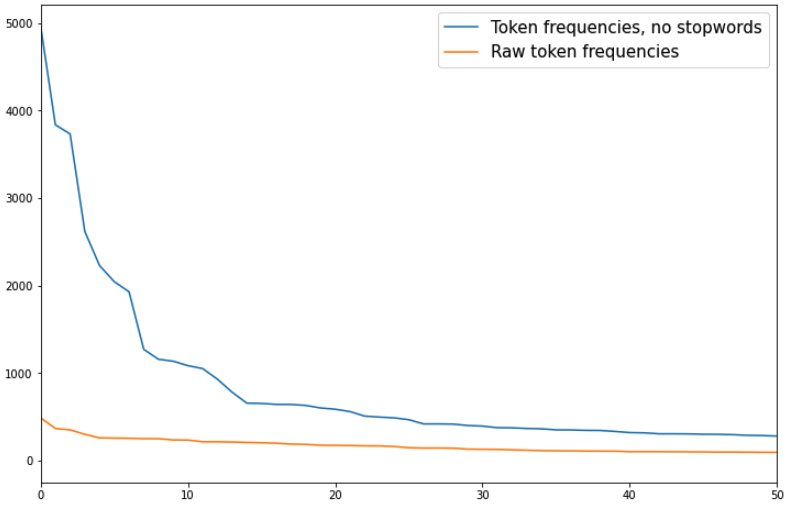
\includegraphics[width=1\linewidth]{imgs/stopwords.png}
  \caption{Token frequencies in training data before and after 
  stopwords removed from the dataset}%
  \label{fig:stopwords}
  \vspace{-10pt}
\end{figure}
%%%%%%%%%%%%%%%%%%%%%%%%%%%%%%%%%%%%%%%%%%%%%%%%%%%%

While this simple experiment gave us insight into the distribution of the token frequencies, we know little of vocabulary size. As mentioned in the introduction, several techniques exist to reduce vocabulary size and preserve meaning. A subset of these were applied to the input data, and the results are displayed in Figure \ref{fig:imgs/token_filter}. After regex separation, several additional filters are applied to the training data, where it can be seen that many tokens occur only once.

%%%%%%%%%%%%%%%%%%%%%%%%%%%%%%%%%%%%%%%%%%%%%%%%%%%%
% Token dimensionality exploration
%%%%%%%%%%%%%%%%%%%%%%%%%%%%%%%%%%%%%%%%%%%%%%%%%%%%
\begin{figure}[htpb]
  \centering
  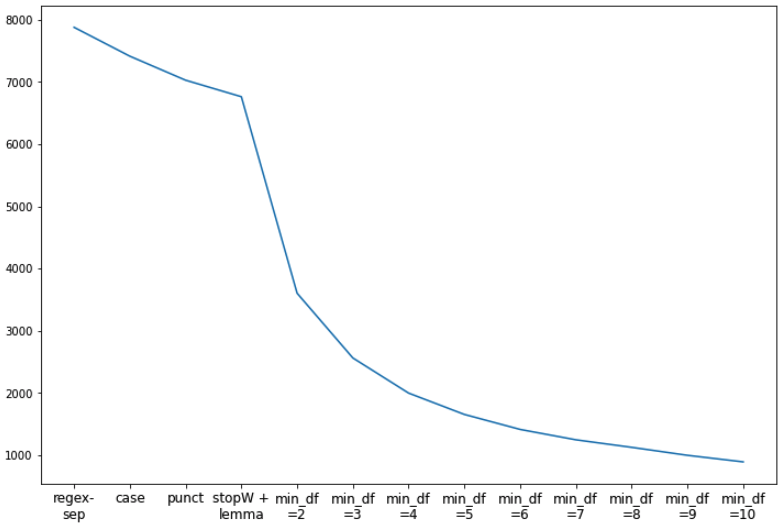
\includegraphics[width=1\linewidth]{imgs/token_filter.png}
  \caption{Vocabulary size as successive filters applied to input corpus. 
    From left to right, the strings are regex separated, then case and
  punctuation is resolved, with final filters trimming rare tokens}
  \label{fig:imgs/token_filter}
  \vspace{-10pt}
\end{figure}
%%%%%%%%%%%%%%%%%%%%%%%%%%%%%%%%%%%%%%%%%%%%%%%%%%%%

To test different theories about the impact of feature engineering on classification, we ran a grid search of several different preprocessing methods on a standard implementation of Logistic Regression (lbfgs solver with L2 loss). Specifically, we leveraged two different tokenization strategies: a conservative regex tokenization from Scikit-Learn's \texttt{CountVectorizer} and a more sophisticated method from Python's \texttt{NLTK Toolkit}. In addition, we also resolved the case of characters and removed punctuation. Finally, lemmatization, or deconjugating words, was applied, as was the removal of stopwords. Once these were completed, vectors were generated from the tokens with two methods: the traditional bag-of-words \cite {luhn1957statistical} count vectorization, and tf-idf vectorization. Tf-idf, or term-frequency inverse document frequency \cite{jones1972statistical}, extends on the bag of words notion by upweighting terms that do not appear in many documents and vice versa. That is, if a term occurs rarely across documents, it should be upweighted as it may prove more predictive.


%%%%%%%%%%%%%%%%%%%%%%%%%%%%%%%%%%%%%%%%%%%%%%%%%%%%
% Feature engineering grid search table
%%%%%%%%%%%%%%%%%%%%%%%%%%%%%%%%%%%%%%%%%%%%%%%%%%%%
\FloatBarrier
\begin{table}[h]
    \centering
    \caption{Feature Engineering Grid Search}
    \begin{tabular}{
    	l
        l
        l
        l
        l
        l
        }
        \toprule
        \multicolumn{2}{c}{} &
        \multicolumn{4}{c}{Token Filters}\\
        \cmidrule(lr){3-6} 
        {Token}& {Tok.} &{None} &{Case+}&{Lem.}& {Stop}\\
        {Engine} & {Sep.} && {Punct.}&&{Word}\\
        \midrule
      CVect & nltk & 0.399& \textbf{0.435}& \textbf{0.435}& 0.401\\
        CVect & reg& 0.396& 0.413&0.413& 0.399\\
        Tf-Idf & nltk & 0.382&  0.382 &0.382 & 0.386\\
        Tf-Idf & reg & 0.360& 0.374 & 0.374& 0.381\\
        \bottomrule
    \end{tabular}
\end{table}
\FloatBarrier
%%%%%%%%%%%%%%%%%%%%%%%%%%%%%%%%%%%%%%%%%%%%%%%%%%%%

Displayed in Table 1, the removal of stopwords tended to, surprisingly, hinder performance. Tf-idf vectorization also performed worse in all cases, running counter to expectations. These two phenomena may be due to the fact that the filler words a candidate uses are somewhat unique to their speaking style and therefore predictive. Less surprisingly, nltk's more sophisticated tokenization engine outperformed its regex counterpart, perhaps due to how it handles intelligently separates contractions (breaking \texttt{can't} into \texttt{ca} + \texttt{n't}). This grid search led to a boost of 2.7\% and 2.1\% over the validation and testing baselines, respectively. 

%%%%%%%%%%%%%%%%%%%%%%%%%%%%%%%%%%%%%%%%%%%%%%%%%%%%
% Dimensionality Reduction
%%%%%%%%%%%%%%%%%%%%%%%%%%%%%%%%%%%%%%%%%%%%%%%%%%%%
\subsection{Dimensionality Reduction}%
\label{sub:dimensionality_reduction}
%%%%%%%%%%%%%%%%%%%%%%%%%%%%%%%%%%%%%%%%%%%%%%%%%%%%

While one method of dimensionality reduction in NLP focuses on trimming out words with little predictive value, the results from feature engineering encouraged us to intregrate all tokens if possible. Therefore, we leveraged Truncated SVD, a matrix decomposition method amenable to sparse data, to generate more semantic features without needing explicitly remove tokens. Below, we ran Truncated SVD across the features generated previously for an increasing number of components. With only 2500 components, roughly a third of the original vocabulary, we were able to exceed our previous performance on the held-out validation set (denoted with a red dotted line). Normalizing token counts before SVD had a negative effect on performance. 


%%%%%%%%%%%%%%%%%%%%%%%%%%%%%%%%%%%%%%%%%%%%%%%%%%%%
% Dimensionality Rediction Figure
%%%%%%%%%%%%%%%%%%%%%%%%%%%%%%%%%%%%%%%%%%%%%%%%%%%%
\begin{figure}[htpb]
  \centering
  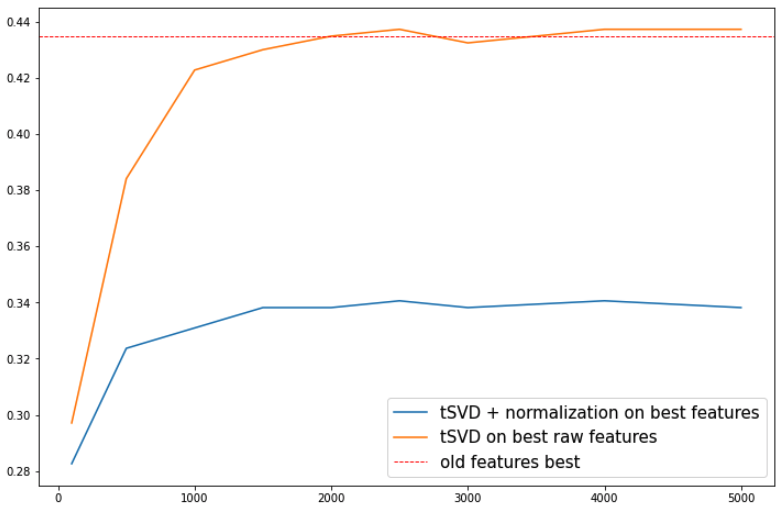
\includegraphics[width=1\linewidth]{imgs/tsvd.png}
  \caption{Classification performance applied to best feature
  selection after Truncated SVD applied with varying numbers of 
 components}%
  \label{fig:tsvd}
  \vspace{-10pt}
\end{figure}
%%%%%%%%%%%%%%%%%%%%%%%%%%%%%%%%%%%%%%%%%%%%%%%%%%%%



%%%%%%%%%%%%%%%%%%%%%%%%%%%%%%%%%%%%%%%%%%%%%%%%%%%%
% Model Ablation
%%%%%%%%%%%%%%%%%%%%%%%%%%%%%%%%%%%%%%%%%%%%%%%%%%%
\subsection{Model Tuning}%
\label{sub:model_tuning}

%%%%%%%%%%%%%%%%%%%%%%%%%%%%%%%%%%%%%%%%%%%%%%%%%%%%

With a smaller set of features and boosted performance on the baseline model, we turned our attention to model tuning directly. Concerned with the effect of dimensionality on the Logistic Regression, we explored regularization with L1 and L2 loss. For comparison, we also ran a trial where no regularization was applied.

%%%%%%%%%%%%%%%%%%%%%%%%%%%%%%%%%%%%%%%%%%%%%%%%%%%%
% Model Grid Search Plot
%%%%%%%%%%%%%%%%%%%%%%%%%%%%%%%%%%%%%%%%%%%%%%%%%%%%
\begin{table}[h]
    \centering
    \caption{Model Tuning: Logistic Regression}
    \begin{tabular}{
    	l
        l
        l
        l
        l
        l
        }
        \toprule
        \multicolumn{1}{c}{} &
        \multicolumn{5}{c}{Logistic Reg. Solver}\\
        \cmidrule(lr){2-6} 
        {Reg.}& {lbfgs} &{lib-} &{newton}&{saga}& {sag}\\
        {Pen.} & {} &{linear}& {}&&{}\\
        \midrule
        - & 0.399 & - & 0.401 & \textbf{0.454} & 0.447\\
        L1 & - & 0.423 &  -&0.428& -\\
        L2 & 0.436& 0.432& 0.448& 0.447& \textbf{0.450}\\
        \bottomrule
    \end{tabular}
\end{table}
%%%%%%%%%%%%%%%%%%%%%%%%%%%%%%%%%%%%%%%%%%%%%%%%%%%%

In general, L1 loss, which induces sparsity, did not perform as well as L2 (weight decay) regularization. Moreover, the non-regularized model performed well on the validation set but hurt performance on the testing set, it was not as robust as its regularized counterpart. 

%%%%%%%%%%%%%%%%%%%%%%%%%%%%%%%%%%%%%%%%%%%%%%%%%%%%
% Semi-Supervised Learning 
%%%%%%%%%%%%%%%%%%%%%%%%%%%%%%%%%%%%%%%%%%%%%%%%%%%%
\section{Semi-supervised Learning with Word Embeddings}%
\label{sec:semi_supervised_learning_with_word_embeddings}

With our supervised model and data tuned, this section explores methods of incorporating unlabeled data to boost performance. In particular, we explore Word2Vec 
embeddings to encode semantic meaning between tokens.
%%%%%%%%%%%%%%%%%%%%%%%%%%%%%%%%%%%%%%%%%%%%%%%%%%%%
% Word2Vec
%%%%%%%%%%%%%%%%%%%%%%%%%%%%%%%%%%%%%%%%%%%%%%%%%%%%
\subsection{Word2Vec for Text Classification}%
\label{sub:word2vec_for_text_classification}

Word2Vec \cite{mikolov2013distributed} is a vectorization method that seeks to embed words that co-occur together, assuming word proximity implies shared meaning \cite{lilleberg2015support}. In our implementation we use a window of 5, meaning the two words to the left and right of a target word are considered during the embedding process. More interesting, this method implicitly downsamples more frequent words, effectively handling the influence of stopwords. As shown in Figure \ref{fig:imgs/w2v_pca}, a Principal Component Analysis (PCA) decomposition a selection of word embeddings, candidates tend to be co-located together, as do words grouped by topic, like conflict or health. 


%%%%%%%%%%%%%%%%%%%%%%%%%%%%%%%%%%%%%%%%%%%%%%%%%%%%
% Word2Vec PCA example
%%%%%%%%%%%%%%%%%%%%%%%%%%%%%%%%%%%%%%%%%%%%%%%%%%%%
\begin{figure}[htpb]
  \centering
  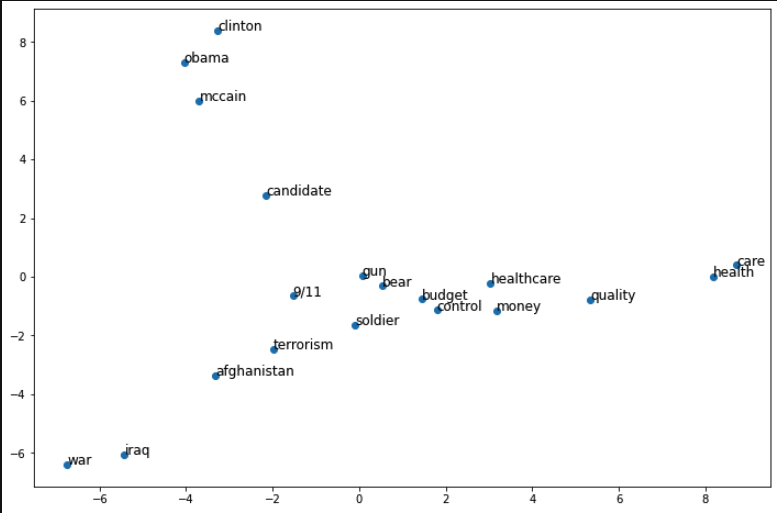
\includegraphics[width=1\linewidth]{imgs/w2v_pca.png}
  \caption{Visualization of Word2Vec embeddings with PCA with a selection 
  of common political terms. Embeddings appear to capture semantic meaning}%
  \label{fig:imgs/w2v_pca}
  \vspace{-8pt}
\end{figure}

%%%%%%%%%%%%%%%%%%%%%%%%%%%%%%%%%%%%%%%%%%%%%%%%%%%%

We chose to utilize word embedding models over the alternatives because we felt it would better generalize similarity in meaning between tokens and boost performance. Other implementations considered include dataset augmentation with unlabeled data. Though a promising option, we were concerned the approach would cause the trained model to diverge under its own, imperfect predictions, leading to poor performance. 


%%%%%%%%%%%%%%%%%%%%%%%%%%%%%%%%%%%%%%%%%%%%%%%%%%%%
% Results and Discussion
%%%%%%%%%%%%%%%%%%%%%%%%%%%%%%%%%%%%%%%%%%%%%%%%%%%%
\subsection{Experimental Results and Discussion}%
\label{subseq:experimental_results_and_discussion}

Given a large corpus of 43,000+ unlabeled speech snippets, we then trained several Word2Vec modelswith different fractions of the dataset. The embedded dimensionality of these words was set to 300 (a common standard), reducing the original dimensionality by an order of magnitude. To generalize this context to documents, the word embeddings in the document are averaged, an order agnostic but somewhat performant approach \cite{turney2010frequency}. Taken alone, these document embeddings were not able to come close to even the initial baseline performance, but increasing the document fraction of the Word2Vec model did improve performance in almost all cases, peaking at 0.34 when all unlabeled data is used.

We think one potential reason the Word2Vec embeddings alone did not meet previous performance is due to its averaging of word embeddings to make document vectors. Since documents are composed of token sequences of varying length, it is typically not useful to sum the embeddings. Averaging these embeddings overcomes this issue, but carries the cost of diluting document meaning across many tokens. Since many presidential candidates speak on similar topics, there may only be subtle differences in the composite embeddings. This is verified by looking at the embeddings of documents taken from the primary speeches of Obama and Clinton, the two most common classes in the dataset, displayed in Figure \ref{fig:imgs/PCA_w2v_Obama}. 


%%%%%%%%%%%%%%%%%%%%%%%%%%%%%%%%%%%%%%%%%%%%%%%%%%%%
% Word2Vec Candidate Embeddings
%%%%%%%%%%%%%%%%%%%%%%%%%%%%%%%%%%%%%%%%%%%%%%%%%%%%
\begin{figure}[htpb]
  \centering
  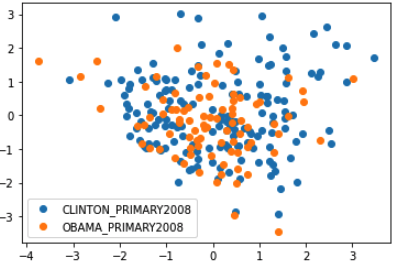
\includegraphics[width=1\linewidth]{imgs/PCA_w2v_Obama.png}
  \caption{Visualization of political candidate embedding profiles
  as defined by their speech embeddings. Little separation can be cleaned,
likely because order is not considered in embedding creation and candidates discuss similar topics}%
  \label{fig:imgs/PCA_w2v_Obama}
  \vspace{-10pt}
\end{figure}
%%%%%%%%%%%%%%%%%%%%%%%%%%%%%%%%%%%%%%%%%%%%%%%%%%%%

Examining this phenomena further, we find that among the 100 most common phrases tied to the tokens \texttt{obama} and \texttt{clinton}, half were shared. Much of what these candidates discuss is interrelated, as expected in a presidential race. With that said, there are still several defining features the embedding model discerned. Notably, the model tied the prases \texttt{tony}, \texttt{foreigner}, and \texttt{president} strongly to Obama but not Clinton. \texttt{tony} refers to Tony Rezko, an Obama fundraiser who was sentenced to prison, while the other features refer to comments about his citizenship and his ascent to president. By contrast, for Hillary Clinton, words such as \texttt{bubba} allude to her campaign to win the vote of white men in the southern United States.

There is considerable overlap in what the two candidates discussed, as described by their document embeddings mapped down to two dimensions. Thus, to differentiate candidates more effectively, these 300-dimensional embeddings were concatenated with the SVD features of the previous analysis. By incorporating semi-supervised embeddings with labeled data, we explored performance changes with our tuned model.

%%%%%%%%%%%%%%%%%%%%%%%%%%%%%%%%%%%%%%%%%%%%%%%%%%%%
% Word2Vec Performance
%%%%%%%%%%%%%%%%%%%%%%%%%%%%%%%%%%%%%%%%%%%%%%%%%%%%
  \vspace{-10pt}
\begin{figure}[htpb]
  \centering
  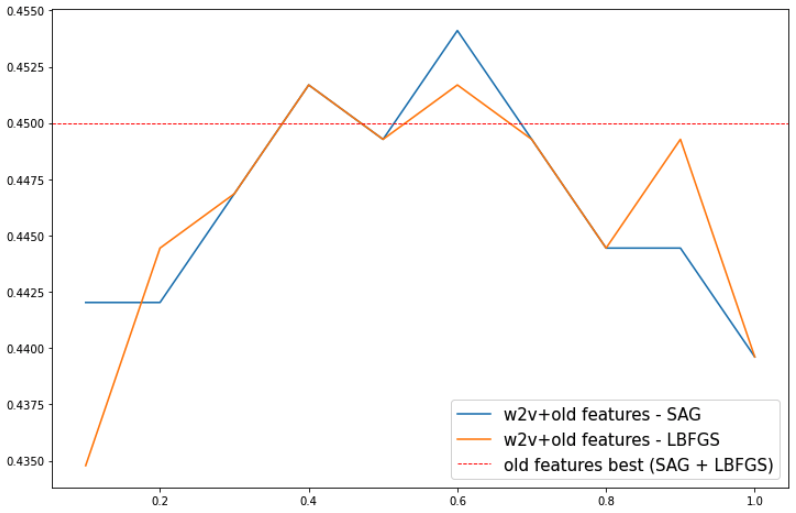
\includegraphics[width=1\linewidth]{imgs/w2v_classification.png}
  \caption{Performance with concatenated Word2Vec document embeddings and different fractions of unlabeled documents and SAG, LBFGS gradient solvers}
  \label{fig:imgs/w2v_classification}
  \vspace{-11pt}
\end{figure}
%%%%%%%%%%%%%%%%%%%%%%%%%%%%%%%%%%%%%%%%%%%%%%%%%%%%

Visualized in Figure \ref{fig:imgs/w2v_classification}, Word2Vec models that were trained on 60\%of the unlabeled data proved optimal for downstream classification. It is surprising to see that performance decreased as the fraction of unlabeled data utilized exceeded 60\%, and may be due to randomness or spurious interactions between our original and embedded data representations. Regardless, the performance on our validation set was again improved, though unfortunately this boost in performance did not translate to the validation set, though it exceeded the baseline.

We can also explore performance more closely with a few examples. In one document, the phrase \texttt{when Bill asks what time it is} was first predicted to be said by Obama, as the word \texttt{Bill} (Bill Clinton) was conflated with legislation. The Word2Vec model disambiguated this issue and correctly predicted Hillary Clinton, who was speaking of her husband. Unfortunately, this extra context was not always helpful. The phrase \texttt{the comatose stance, "Re-elect Obama"}, stated as criticism of Democrats by Newt Gingrich, was misinterpreted by the additional context that Democrats supported Obama in his bid for re-election in 2012. Instead of predicting Gingrich, the model now associated the phrase with Hillary Clinton, a vocal proponent of the Democratic party.


%%%%%%%%%%%%%%%%%%%%%%%%%%%%%%%%%%%%%%%%%%%%%%%%%%%%
% Conclusion
%%%%%%%%%%%%%%%%%%%%%%%%%%%%%%%%%%%%%%%%%%%%%%%%%%%%
\section{Conclusion}%
\label{sec:conclusion}

Through a sequence of grid search explorations, model tuning, and contextual word embeddings, we were able to improve our classifier beyond the existing baseline. We feel that this can be credited to our consideration of data tokenization, feature engineering, and principled methods for dimensionality reduction. However, the additional context we incorporated was not universally beneficial. In some cases, additional context actually further confused the canonical meaning, usually in cases where flowery or idiomatic language was utilized. However, with context the model improved overall.



%%%%%%%%%%%%%%%%%%%%%%%%%%%%%%%%%%%%%%%%%%%%%%%%%%%%

%%%%%%%%%%%%%%%%%%%%%%%%%%%%%%%%%%%%%%%%%%%%%%%%%%%%
% Statement of Collaboration
%%%%%%%%%%%%%%%%%%%%%%%%%%%%%%%%%%%%%%%%%%%%%%%%%%%%
\section{Statement of Collaboration}
For this project I utilized a variety of resources. These include articles read from google scholar, API documentation for different NLP packages, and office hours with Dr. Singh. Beyond these resources, I completed this project in isolation and the content within this report is my own.
%%%%%%%%%%%%%%%%%%%%%%%%%%%%%%%%%%%%%%%%%%%%%%%%%%%%



\bibliography{custom}
\bibliographystyle{acl_natbib}

\appendix

%%%%%%%%%%%%%%%%%%%%%%%%%%%%%%%%%%%%%%%%%%%%%%%%%%%%
% Future Research
%%%%%%%%%%%%%%%%%%%%%%%%%%%%%%%%%%%%%%%%%%%%%%%%%%%%
\section{Future Research}%
\label{sec:future_research}
Some potential avenues for future research within the stated constraints of the problem include alternative word embedding strategies such as GloVE \cite{pennington2014glove}. In addition, designing a method to incorporate word order would likely improve the expressivity of our features. This could be as simple as incorporating bigrams or training a sequence \cite{hochreiter1997long} or self-attention \cite{vaswani2017attention} model to keep a memory statistic of the sequence information. External sources of data such as a pretrained embedding model on a larger corpus could be useful as well and fine tuned for our specific objective.


\end{document}% File acl2020.tex

